\documentclass[12pt,a4paper]{article}
\usepackage{iftex}
\ifPDFTeX
\usepackage[T2A]{fontenc}
\usepackage[utf8]{inputenc}
\usepackage[ukrainian]{babel}
\else
\usepackage{fontspec}
\usepackage{polyglossia}
\setdefaultlanguage{ukrainian}
\IfFontExistsTF{DejaVu Serif}{
\setmainfont{DejaVu Serif}
\setsansfont{DejaVu Sans}
\setmonofont{DejaVu Sans Mono}
}{
\IfFontExistsTF{Liberation Serif}{
\setmainfont{Liberation Serif}
\setsansfont{Liberation Sans}
\setmonofont{Liberation Mono}
}{
\setmainfont{Arial}
\setsansfont{Arial}
\setmonofont{Arial}
}
}
\fi
\usepackage[left=22mm,right=18mm,top=20mm,bottom=22mm]{geometry}
\usepackage{graphicx}
\usepackage{booktabs}
\usepackage{array}
\usepackage{tabularx}
\usepackage{float}
\usepackage{xcolor}
\usepackage{listings}
\usepackage{hyperref}
\usepackage{microtype}
\hypersetup{colorlinks=true,linkcolor=blue,urlcolor=blue}
\definecolor{codegray}{RGB}{245,245,245}
\lstset{
basicstyle=\ttfamily\small,
backgroundcolor=\color{codegray},
frame=single,
breaklines=true,
showstringspaces=false
}
\setlength{\parindent}{1.25cm}
\setlength{\parskip}{3pt}

\begin{document}

\begin{titlepage}
\centering
\vspace*{25mm}
{\Large Lab 2. Performance Measurement and Analysis\par}
\vspace{4mm}
{\large Assembler and low-level optimisation\par}
\vfill
{\large Кашинський Владислав\par}
\vspace{2mm}
{\large студент 3-го курсу, група ТТП-32\par}
\vfill
{\large 2026\par}
\end{titlepage}

\tableofcontents
\newpage

\section{Мета роботи}

Мета роботи полягає у вимірюванні продуктивності скомпільованої програми, визначенні найбільш витратних функцій та порівнянні виконання до і після низькорівневої оптимізації. Дослідження виконано у Windows 11 з Visual Studio 2026 та Intel VTune Profiler 2026.4.

Замість Linux perf використано Visual Studio CPU Usage та Intel VTune. Розширену статистику часу зібрано через Windows Process API. Енергію процесорного package виміряно системним лічильником Windows RAPL Energy Meter.

\section{Досліджувана програма}

Програма множить дві квадратні матриці типу \texttt{float}. Для матриці розміру $n$ кількість арифметичних операцій оцінюється як $2n^3$. Розмір матриці та кількість повторів передаються через командний рядок. Після обчислення програма друкує час ядра, GFLOP/s та checksum.

Підготовлено дві збірки:

\begin{table}[H]
\centering
\begin{tabularx}{\textwidth}{@{}lXX@{}}
\toprule
Варіант & Ключі MSVC & Обчислювальне ядро \\
\midrule
Baseline & \texttt{/Od /Ob0} & скалярний цикл \\
Optimized & \texttt{/O2 /arch:AVX2 /fp:fast} & AVX2 та FMA \\
\bottomrule
\end{tabularx}
\caption{Варіанти збірки}
\end{table}

Для обох варіантів використані однакові вхідні дані. Відносна різниця checksum становить $3.96\cdot10^{-9}$, що знаходиться в межах похибки обчислень з рухомою комою.

\section{Час виконання та пам'ять}

Кожну версію запущено п'ять разів з параметрами $n=768$ та $repeats=6$. У таблиці наведені медіанні значення.

\begin{table}[H]
\centering
\begin{tabular}{@{}lrrr@{}}
\toprule
Метрика & Baseline & Optimized & Зміна \\
\midrule
Wall time, s & 7.949043 & 0.467363 & 17.01x \\
Kernel time, s & 7.873978 & 0.446038 & 17.65x \\
CPU time, s & 7.656250 & 0.421875 & 18.15x \\
Peak working set, MiB & 10.652 & 10.652 & 0.00\% \\
GFLOP/s & 0.690 & 12.187 & 17.65x \\
\bottomrule
\end{tabular}
\caption{Результати вимірювання часу}
\end{table}

Оптимізація прискорила обчислювальне ядро у 17.65 раза. Використання пам'яті не змінилося, оскільки обидві версії зберігають однакові три матриці.

\section{Flame Graph}

Flame Graph побудовано у Visual Studio Performance Profiler. Ширина блоку показує частку зібраних CPU samples, а висота відповідає глибині стеку викликів.

\begin{figure}[H]
\centering
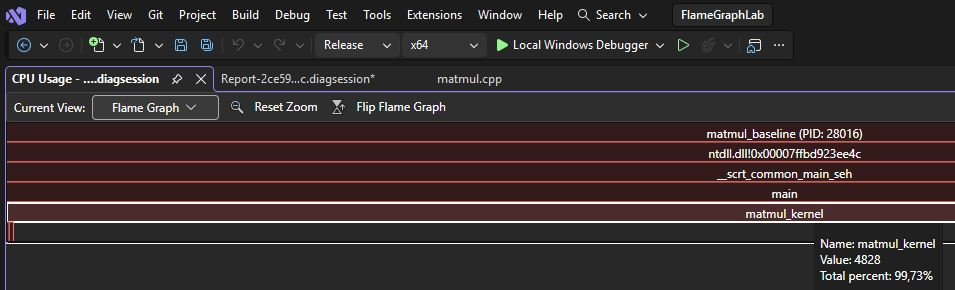
\includegraphics[width=0.98\textwidth]{flamegraph-baseline.jpg}
\caption{Flame Graph baseline}
\end{figure}

У baseline функція \texttt{matmul\_kernel} займає 99.73\% профілю. Це означає, що практично весь процесорний час витрачається на множення матриць.

\begin{figure}[H]
\centering
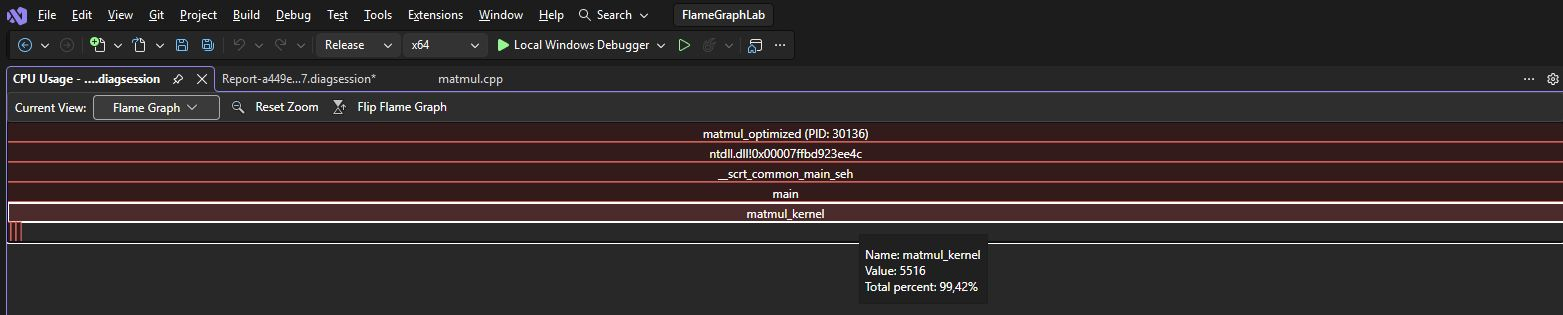
\includegraphics[width=0.98\textwidth]{flamegraph-optimized.jpg}
\caption{Flame Graph optimized}
\end{figure}

В optimized частка \texttt{matmul\_kernel} становить 99.42\%. Відносна ширина залишається великою, але абсолютний час ядра зменшився у 17.65 раза. Кожний Flame Graph нормалізований до тривалості власного запуску, тому його потрібно розглядати разом з числовими вимірюваннями.

\section{Intel VTune Hotspots}

VTune Hotspots використано як аналог \texttt{perf record} та \texttt{perf report}. Для optimized виконано більше повторів, щоб отримати достатню кількість програмних семплів.

\begin{table}[H]
\centering
\begin{tabular}{@{}lrrrr@{}}
\toprule
Варіант & Повтори & Kernel, s & На повтор, s & Частка kernel \\
\midrule
Baseline & 20 & 14.797 & 0.740 & 100.0\% \\
Optimized & 200 & 8.689 & 0.043 & 99.7\% \\
\bottomrule
\end{tabular}
\caption{Результати VTune Hotspots}
\end{table}

В обох профілях \texttt{matmul\_kernel} є головною гарячою функцією. Стек викликів має вигляд \texttt{main -> matmul\_kernel}.

\section{Апаратні лічильники}

Апаратні події зібрано в Intel VTune Microarchitecture Exploration для однакового навантаження $768\times768$, 6 повторів.

\begin{table}[H]
\centering
\begin{tabular}{@{}lrr@{}}
\toprule
Метрика & Baseline & Optimized \\
\midrule
Clockticks & 24,429,378,592 & 3,723,094,384 \\
Instructions Retired & 57,635,114,976 & 2,836,148,506 \\
CPI & 0.424 & 1.313 \\
IPC & 2.359 & 0.762 \\
Back-End Bound, \% & 37.9 & 49.5 \\
Memory Bound, \% & 15.1 & 17.5 \\
FP Scalar, \% & 8.7 & 0.2 \\
256-bit FP Vector, \% & 0.0 & 49.0 \\
Vector Capacity Usage, \% & 6.3 & 49.8 \\
\bottomrule
\end{tabular}
\caption{Результати Microarchitecture Exploration}
\end{table}

Після оптимізації кількість clockticks зменшилася у 6.56 раза, а Instructions Retired у 20.32 раза. Метрики 256-bit FP Vector та Vector Capacity Usage підтверджують використання AVX2. Зростання Memory Bound пояснюється тим, що після прискорення арифметики більшу частку часу займає передавання даних.

\section{Асемблерний код}

У baseline внутрішній цикл містить скалярні операції:

\begin{lstlisting}
movss xmm0, DWORD PTR [rcx+rax*4]
mulss xmm0, DWORD PTR [rax+rcx*4]
addss xmm1, xmm0
\end{lstlisting}

У optimized використані AVX2 та FMA:

\begin{lstlisting}
vbroadcastss ymm1, DWORD PTR [rdi+rax]
vmovups ymm0, YMMWORD PTR [r8+rax*4]
vfmadd213ps ymm0, ymm1, YMMWORD PTR [rdx+rax*4]
vmovups YMMWORD PTR [rdx+rax*4], ymm0
vzeroupper
\end{lstlisting}

Інструкція \texttt{vbroadcastss} заповнює вісім 32-бітних елементів YMM-регістра одним значенням. \texttt{vfmadd213ps} виконує множення і додавання для восьми \texttt{float}. Baseline обробляє один елемент за інструкцію, а optimized обробляє вісім.

\section{Енергоспоживання}

Windows RAPL Energy Meter повертає накопичену енергію процесорного package у піковат-годинах. Різниця показів переведена у джоулі. Для оцінки динамічної енергії програми від енергії workload віднято idle тієї самої тривалості. Виконано п'ять пар вимірювань.

\begin{table}[H]
\centering
\begin{tabular}{@{}lrrrr@{}}
\toprule
Варіант & Package, J & Idle, J & Program, J & Потужність, W \\
\midrule
Baseline & 83.690 & 34.703 & 48.464 & 24.194 \\
Optimized & 6.653 & 2.517 & 4.160 & 27.622 \\
\bottomrule
\end{tabular}
\caption{Медіанні значення енергії одного запуску}
\end{table}

Середня потужність optimized зросла на 14.2\%, але динамічна енергія зменшилася на 91.4\%. Причиною є значне скорочення часу виконання. RAPL вимірює процесорний package, а не повне споживання комп'ютера від розетки.

\section{Висновки}

Оптимізація з AVX2 та FMA прискорила ядро множення матриць у 17.65 раза. VTune показав зменшення кількості виконаних інструкцій у 20.32 раза та підтвердив використання 256-бітних векторних операцій. Flame Graph визначив \texttt{matmul\_kernel} як головну гарячу функцію в обох версіях. Динамічна енергія програми зменшилася з 48.464 J до 4.160 J. Результати baseline та optimized збігаються в межах похибки обчислень з рухомою комою.

\section{Джерела}

\begin{enumerate}
\item Brendan Gregg. CPU Flame Graphs. \url{https://www.brendangregg.com/FlameGraphs/cpuflamegraphs.html}
\item Brendan Gregg. perf Examples. \url{https://www.brendangregg.com/perf.html}
\item Microsoft. Flame Graph. \url{https://learn.microsoft.com/en-us/visualstudio/profiling/flame-graph}
\item Intel. VTune Profiler User Guide. \url{https://www.intel.com/content/www/us/en/docs/vtune-profiler/}
\item Microsoft. Energy Meter Interface. \url{https://learn.microsoft.com/en-us/windows-hardware/drivers/powermeter/energy-meter-interface}
\end{enumerate}

\end{document}

